%!TEX root = ../main.tex
\section{Experiments}
\label{sec:exp}

We conduct preliminary experiments to demonstrate the effectiveness of \sys. 
We evaluate its performance in two key processes: Reasoning and Verification. %The multimodal data lakes and data discovery techniques used in these experiments are discussed respectively for each process. 

%\subsection{Question Answering using Retrieved Multimodal Data}

%To validate the effectiveness of our method in text reasoning and mutimodal (text+image) reasoning, we design the experiment on natural language question answering and visual-based entity question answering.

\subsection{Question Answering}

\stitle{Experiment Setting.} In this experiment, we focus on evaluating question answering performance using a multimodal data lake consisting of 400K web tables and 6M English passages extracted from Wikipedia. The data lake includes both tables and texts, and each query is designed to retrieve relevant data items to answer a given question. We use 18 manually crafted user queries, each with corresponding ground truth annotations specifying the required data items, sub-queries for decomposition, and final answers.

\stitle{Data Discovery Evaluation.}
The effectiveness of data discovery is measured using the recall at $K$ (R@$K$) metric, which calculates the proportion of relevant data items retrieved in the top-$K$ recommendations. The experimental results show that when $K$ is 5, 10, 15, and 20, the R@$K$ values are 40.8\%, 46.3\%, 59.3\%, and 77.8\%, respectively. For 12 out of the 18 queries, \sys successfully discovers all the relevant items needed to answer the query. The remaining 6 queries show partial success. In total, 30 out of 38 related items are correctly discovered, demonstrating the potential of the proposed data discovery methodology, even though it is still in a preliminary stage.


\stitle{Query Decomposition Evaluation.}
To decompose queries into manageable sub-queries, \sys serializes the discovered data items and uses GPT-3 to generate sub-queries. The output includes the sub-queries and corresponding data item ids. Evaluation of the decomposition quality is based on two criteria: (1) whether each sub-query is useful for solving the original query, and (2) whether the sub-query can be answered correctly using the selected data item. The human evaluation results show that 77.8\% of the queries scored 2 (both criteria met), 16.7\% scored 1 (only the first criterion met), and 5.5\% scored 0. 

Table~\ref{tab:results_of_decomposition} shows the results of 8 instances. \sys is able to handle different aggregation operations, such as sum (Instance 2) and comparison (Instance 3). Further, it correctly understands long sentences (Instance 1). However, \sys has difficulty in dealing with sentences with complex syntactic structures (\eg in Instance 4, GPT-3 mistakenly generates $q_3$ because it takes the subject of released'' as Academy Award for Best Foreign Language Film''.). 


\begin{table}[!t]
\centering
\resizebox{\textwidth}{!}{
{\small
\begin{tabular}{p{15cm}}
\hline
\underline{Instance 1}: $Q$: Did the 2014 United States house of representatives elections take place on the same day in Rhode Island, South Carolina and Louisiana? $E = \{P_1, P_2, P_3\}$\\
$\rightarrow$ $q_1$: Did the 2014 United States House of Representatives elections take place on November 4, 2014 in Rhode Island? $e_1 = P_1$; $q_2$: Did the 2014 United States House of Representatives elections take place on November 4, 2014 in South Carolina? $e_2 = P_2$; $q_3$: Did the 2014 United States House of Representatives elections take place on November 4, 2014 in Louisiana? $e_3 = P_3$ \\
$\bigstar$ Score: 2 \\
\hline
\underline{Instance 2}: $Q$: How many representatives were elected in the 2014 United States house of representatives elections in Rhode Island and South Carolina?   %\srm{Question is vague, are we asking for a sum?}
$E = \{P_1, P_2\}$ \\
$\rightarrow$ $q_1$: How many representatives were elected in the 2014 United States house of representatives elections in Rhode Island? $e_1 = P_1$; $q_2$: How many representatives were elected in the 2014 United States house of representatives elections in South Carolina? $e_2 = P_2$ \\
$\bigstar$ Score: 2 \\
\hline
\underline{Instance 3}: $Q$: Which number is larger, the number of living former prime ministers of Tunisia or the number of former presidents of Ghana? $E = \{T_1, P_1\}$ \\
$\rightarrow$ $q_1$: What is the number of living former prime ministers of Tunisia? $e_1 = P_1$; $q_2$: What is the number of former presidents of Ghana? $e_2 = T_1$ \\
$\bigstar$ Score: 2 \\
\hline
\underline{Instance 4}: $Q$: What year was the first German film that won the Academy Award for Best Foreign Language Film released? $E = \{T_1, P_1\}$ \\
$\rightarrow$ $q_1$: What year was the film The Tin Drum released? $e_1 = T_1$; $q_2$: What was the first German film that won the Academy Award for Best Foreign Language Film? $e_2 = T_1$; $q_3$: What year was the first Academy Award for Best Foreign Language Film given out? $e_3 = T_1$ \\
$\bigstar$ Score: 0 \\
\hline
\underline{Instance 5}: $Q$: Did The Tin Drum and Kolya both win the Academy Awards for Best Foreign Language Film? $E = \{P_1, P_2\}$ \\
$\rightarrow$ $q_1$: whether The Tin Drum has ever won the Academy Award for Best Foreign Language Film? $e_1 = P_1$; $q_2$: whether Kolya has ever won the Academy Award for Best Foreign Language Film? $e_2 = P_2$ \\
$\bigstar$ Score: 2 \\
\hline
\underline{Instance 6}: $Q$: How many years elapsed between the premiere of season 10 and the premiere of season 5 of Law \& Order : Special Victims Unit? $E = \{T_1, T_2\}$ \\
$\rightarrow$ $q_1$: What is the premiere date of season 10 of Law \& Order : Special Victims Unit? $e_1 = T_2$; $q_2$: What is the premiere date of season 5 of Law \& Order : Special Victims Unit? $e_1 = T_1$ \\
$\bigstar$ Score: 2 \\
\hline
\underline{Instance 7}: $Q$: Did You Let Me Walk Alone participate in the Eurovision Song Contest in 1996? $E = \{T_1, P_1\}$ \\
$\rightarrow$ $q_1$: What year was the Eurovision Song Contest held in Lisbon, Portugal? $e_1 = T_1$; $q_2$: What year was You Let Me Walk Alone released? $e_2 = P_1$ \\
$\bigstar$ Score: 1 \\
\hline
\underline{Instance 8}: $Q$: Are the tallest building in the united kingdom and the tallest building in poland above 200 meters? $E = \{T_1, T_2\}$\\
$\rightarrow$ $q_1$: What is the height of the tallest building in the United Kingdom? $e_1 = T_1$; $q_2$: What is the height of the tallest building in Poland? $e_2 = T_2$ \\
$\bigstar$ Score: 2 \\
\hline
\end{tabular}
}
}
\caption{Example sub-queries generated by \sys. $q_i$ and $e_i$ represent the $i_{th}$ sub-query and its corresponding data item. $T_i$ represents a table and $P_i$ represents a text. 
}
\label{tab:results_of_decomposition}
\end{table}


% \subsubsection{Visual-based Entity Question Answering}

% \stitle{Experiment Setting.}
% The experiments were conducted in a zero-shot setting using RTX 4090 GPUs. For GPT-4V, we used the interface of the GPT-4-vision-preview model. It's worth noting that GPT-4V often refrains from answering person identify questions without additional clues due to policy reasons. However, with the incorporation of matching graph techniques, it can leverage weak signals and combine them with its own knowledge base. For the dataset, we chose NewsPersonQA~\cite{zhang2024mar}. For the task evaluation, we use accuracy (\textbf{Acc}) as an evaluation metric. Furthermore, we assess the accuracy only for instances where relevant clues are successfully retrieved, which is denoted as \textbf{Acc}$^{{hit}}$.

% \stitle{Baseline.} For answering queries, we selected two well-known and highly capable MLLMs, as well as human evaluation,to serve as baselines. \textbf{LLaVA:} 
% This model utilizes CLIP-ViT-L-336px with an MLP projection. We refer to the 1.5 version with 7 billion parameters as LLaVA-7b and the version with 13 billion parameters as LLaVA-13b.
% \textbf{GPT-4V:} 
% Recognized as OpenAI's most powerful general-purpose MLLM to date, GPT-4V boasts 1.37 trillion parameters. 

% \stitle{Main Results.} The main results of visual-based entity question answering are summarized in Table~\ref{tbl:single}, which leads to the following insights: LLaVA-13b demonstrates higher accuracy (27.93\%) compared to LLaVA-7b (22.26\%), suggesting that a model's recognition ability is positively correlated with its parameter size, which to some extent reflects its knowledge base. Incorporating a matching graph leads to an 8.9\% improvement in accuracy for LLaVA-7b and a 3.2\% improvement for LLaVA-13b. GPT-4V, with matching, achieves a character recognition accuracy of 34.83\%.
%  The enhancement from matching is more pronounced for LLaVA-7b than for LLaVA-13b, indicating that while matching can compensate for differences in parameters, a model's inherent capabilities still set an upper limit on its performance.

% \begin{table}[t!]
% \caption{Result for Visual-based Entity Question Answering. (Note: GPT-4V could not answer these queries directly due to policy constraints. Values within parentheses are those GPT-4V still refuses to answer.)}
% \small
% \centering
% \label{tbl:single}
% \resizebox{0.5\columnwidth}{!}{
% \begin{tabular}{l|l|l}
% \toprule
% {\textbf{Models}}     & \textbf{Acc} (\%) & \textbf{Acc}$^{{hit}}$ (\%) \\ 
% \midrule
% \textbf{LLaVA-7b}                        & 22.26        & 27.53         \\
% {\textbf{LLaVA-7b + Symphony}} & 31.19        & 62.81         \\ 
% \hline
% \textbf{LLaVA-13b}                       & 27.93        & 32.86         \\
% {\textbf{LLaVA-13b + Symphony}} & 31.13        & 62.34         \\ 
% \hline
% \textbf{GPT-4V}                          & -            & -             \\
% {\textbf{GPT-4V + Symphony}} & 34.84 (4.2)  & 68.31 (2.6)  \\ 
% \midrule
% \textbf{Symphony(Graph Reasoning)}                            & {\bf 39.09}        & {\bf 79.65}         \\ 
% \bottomrule
% \end{tabular}
% }
% \end{table}


\subsection{Answer Verification}

We showcase preliminary experimental results that highlight the initial achievements of \sys in facilitating the verification of generative AI. 
% \yang{Do we need to include tuple-tuple and text generation?}

\stitle{Experiment Setting.}
We perform a controlled study to assess textual claims, employing 1,300 textual claims from the TabFact~\cite{chen2019tabfact} benchmark, which is currently the most advanced benchmark for verifying the credibility of textual hypotheses by utilizing a given table. The data lake consists of 16,573 tables from the TabFact and 2,925 tables sourced from WikiTable-TURL~\cite{deng2022turl}.


\begin{figure}[t!]
\vspace{1em}
\begin{center}
  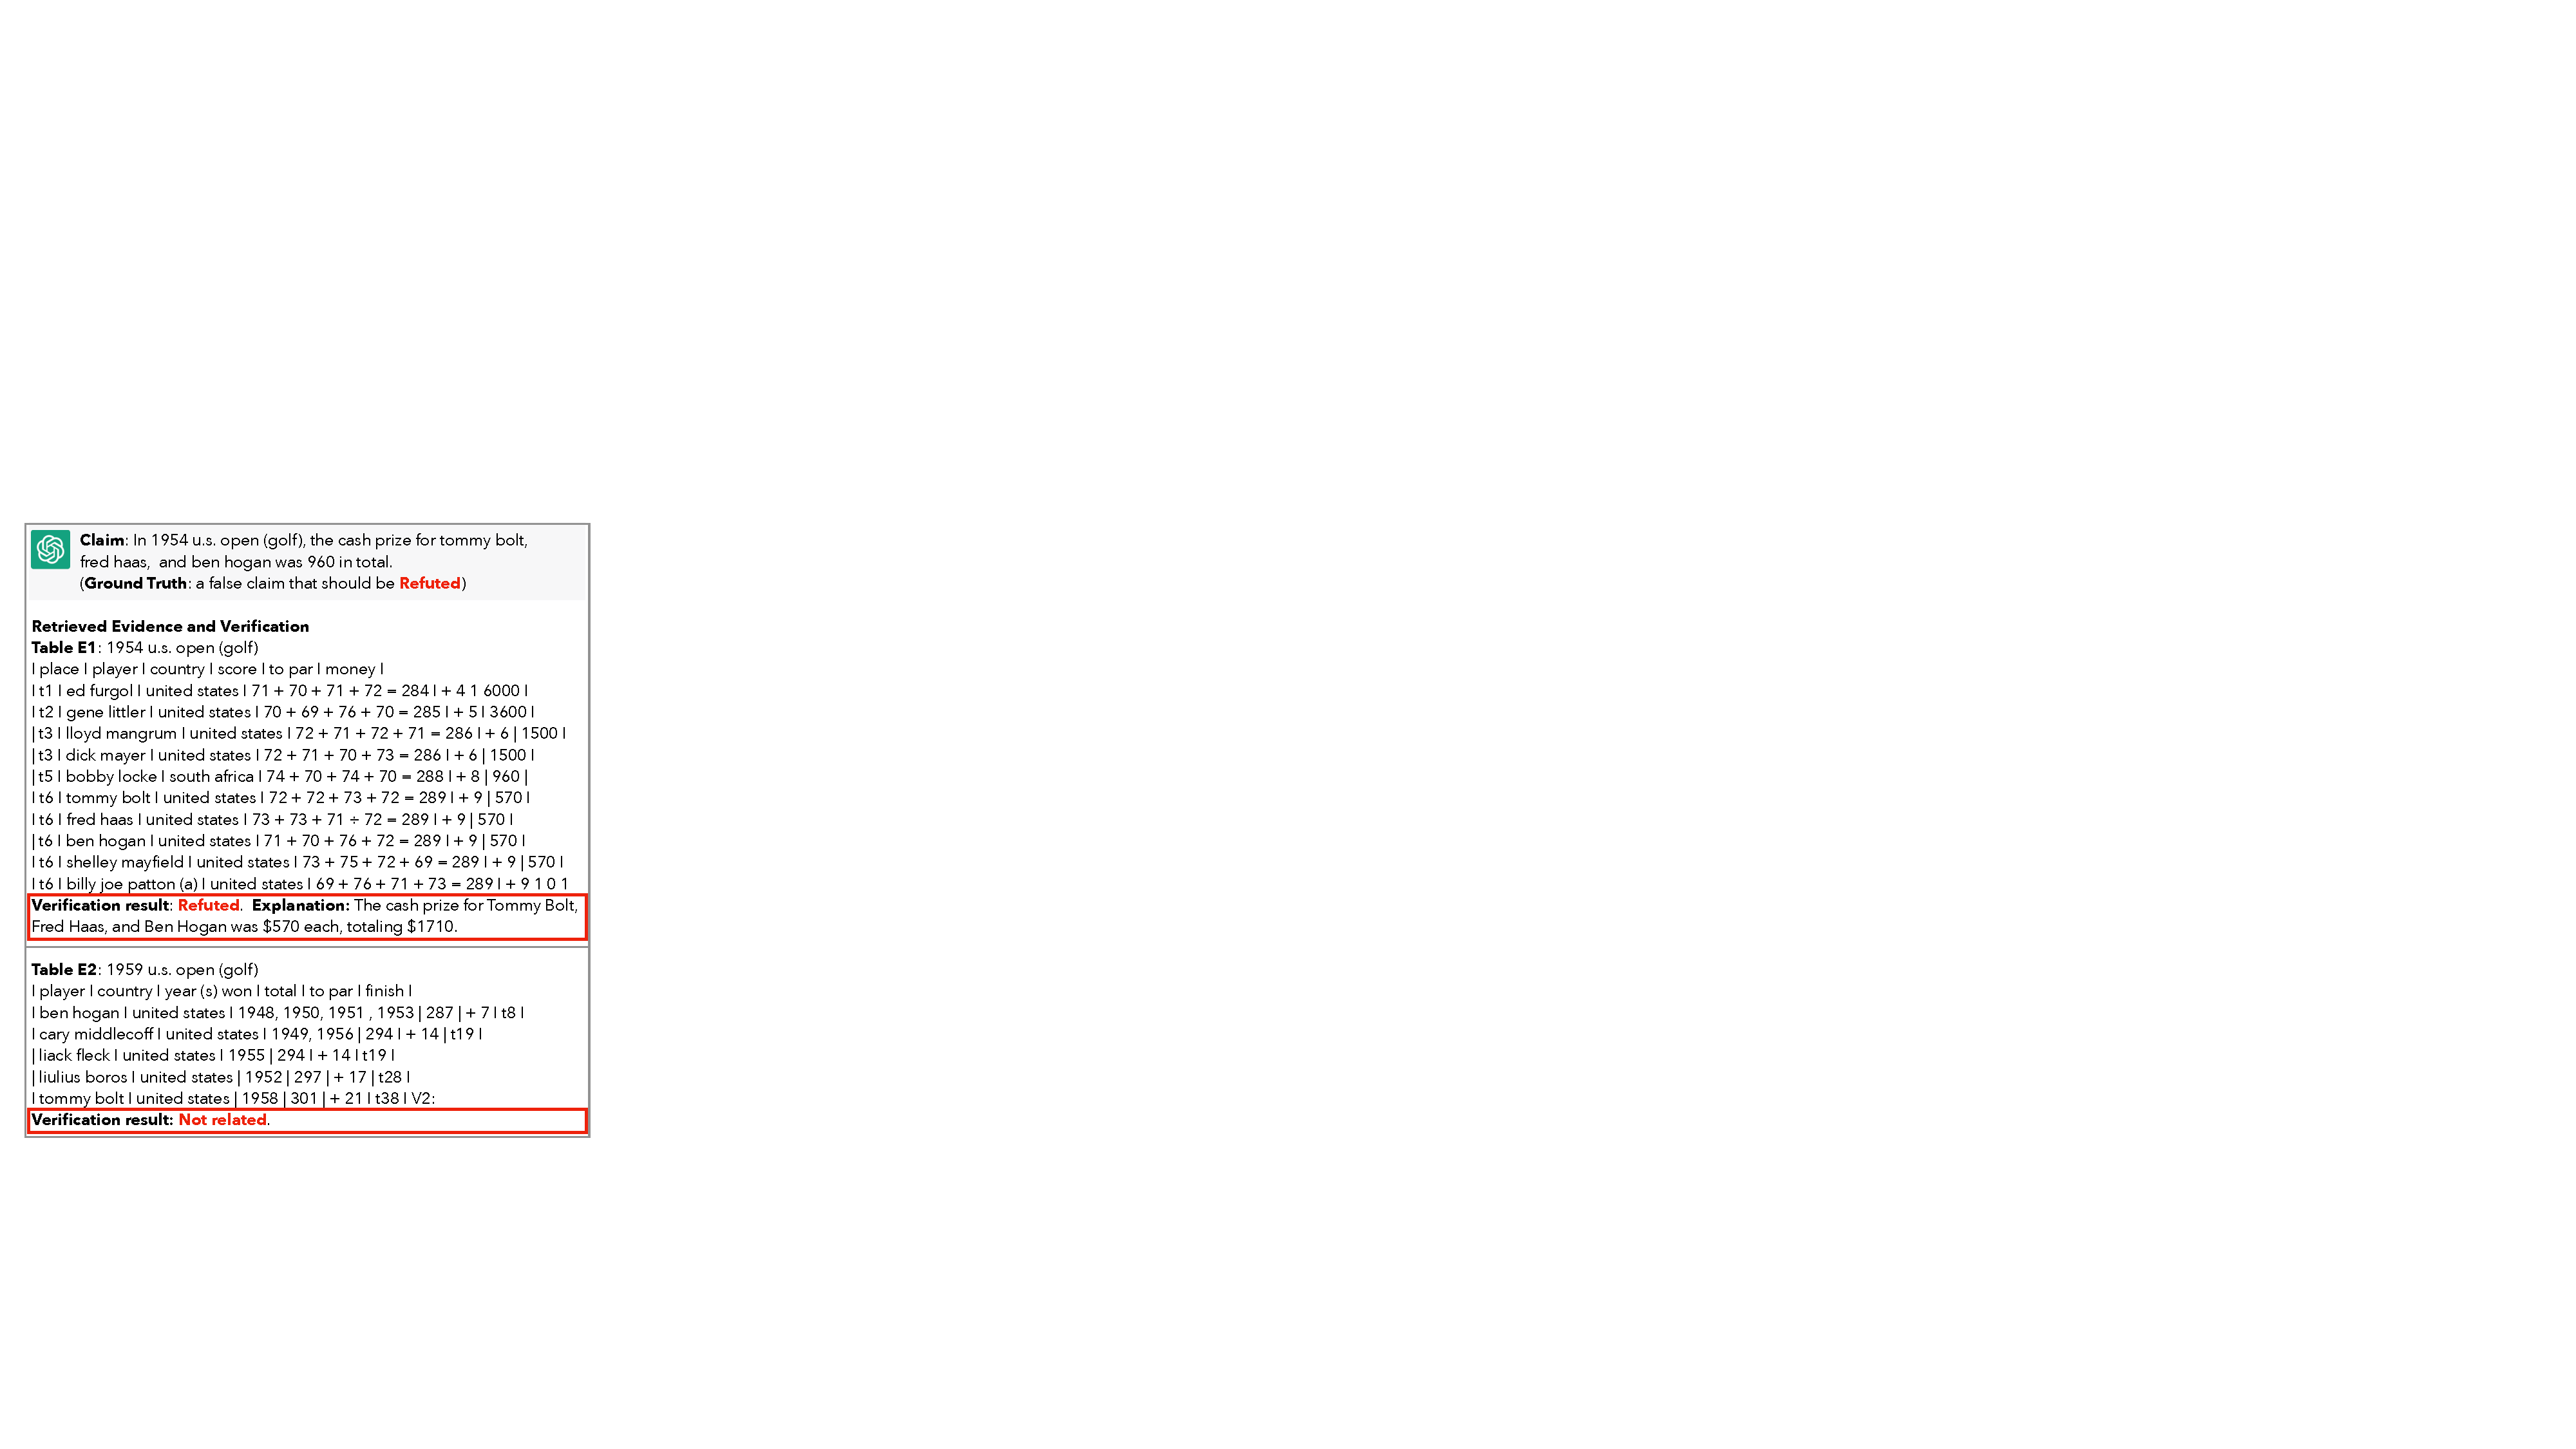
\includegraphics[width=0.65\textwidth]{submissions/Nan2024/figs/tabfact.pdf}
  \caption{Verifying a textual claim using retrieved tables.}
  \label{fig:claim_case} 
\end{center}
\end{figure}


\stitle{Evaluation for Retrieval.} 
We use Elasticsearch~\cite{elasticsearch} to retrieve the top-5 tables for each textual claim. Given the limited amount of relevant data, we focus on the recall metric for evaluation. Each textual claim is associated with a corresponding table in the original dataset, which we consider relevant evidence, while other retrieved tables are deemed irrelevant. The retrieval performance, measured by R@5, is 0.88.

\stitle{Evaluation for Verification.} 
We evaluate the verification process using two different verifiers: GPT-3.5, the default verifier for both data types, and PASTA~\cite{pasta}, a specialized model for text verification.
%
The performance of the verifiers is measured by accuracy. When the retrieved data cannot support or refute a claim, the verifier outputs ``not related''. However, in this case, since PASTA that only offers two different answers: ``true'' or ``false'', we consider it's also correct when PASTA outputs ``false''.

We conduct experiments in two settings. When a relevant table is retrieved and provided as evidence to the verifier, PASTA achieves higher accuracy than GPT-3.5 (0.89 vs. 0.75) in verifying the textual claim based on the table. However, in cases where many of the retrieved tables are irrelevant to the claim, the verifier must accurately determine which tables are not related. In this setting, PASTA's accuracy drops to 0.72 because it has not encountered this scenario during training, while GPT-3.5 improves to 0.91. 
% Thus, GPT-3.5-turbo demonstrates superior generalization capabilities and performs better than PASTA when dealing with irrelevant tables.
Thus, when the retrieved data is highly related to the generative data, local models like PASTA have higher accuracy while protecting privacy. In contrast, GPT-3.5 is better at generalizing and providing explanations for further judgments. Users can select the appropriate model based on their requirements.


In Figure~\ref{fig:claim_case}, we present a case of verifying a textual claim based on retrieved tables using GPT-3.5. \sys retrieves two tables $E_1$ and $E_2$, where $E_1$ can be used with an aggregation query to refute the claim while $E_2$ is not related because it is for the year 1959. The red boxes in Figure~\ref{fig:claim_case} show that GPT-3.5 can provide not only a verification result but also some explanation.




